\documentclass[a4paper,10pt]{article}

\input{style/ch_xelatex.tex}
\input{style/scala.tex}
\usepackage{ctex}
\usepackage{graphicx}
\usepackage{amssymb}
\usepackage{enumerate}
\usepackage{xcolor}
\usepackage{bm}
\usepackage{lastpage}
\usepackage{fancyhdr}
\usepackage{tabularx}
\usepackage{geometry}
\usepackage{float}
\usepackage{booktabs}
\usepackage{array}
\usepackage{enumitem}
\usepackage{url}
\usepackage{xurl}
\usepackage{caption}
\usepackage{titlesec}

\geometry{a4paper,left=2.1cm,right=2.1cm,top=2.2cm,bottom=2.2cm}
\pagestyle{fancy}
\lhead{并行程序设计 Lab1 实验报告}
\rhead{体系结构相关编程}
\cfoot{\thepage/\pageref{LastPage}}
\renewcommand{\headrulewidth}{0.3pt}
\setlength{\parskip}{0.22em}
\setlist[itemize]{nosep,leftmargin=1.5em}
\setlist[enumerate]{nosep,leftmargin=1.8em}
\captionsetup{font=small}
\titlespacing*{\section}{0pt}{0.65em}{0.3em}
\titlespacing*{\subsection}{0pt}{0.45em}{0.2em}
\titlespacing*{\subsubsection}{0pt}{0.3em}{0.15em}
\Urlmuskip=0mu plus 1mu\relax
\newcolumntype{P}[1]{>{\raggedright\arraybackslash}p{#1}}
\newcolumntype{Y}{>{\raggedright\arraybackslash}X}

\begin{document}
\renewcommand{\figurename}{图}
\renewcommand{\tablename}{表}
\renewcommand{\today}{\number\year 年 \number\month 月 \number\day 日}

\begin{titlepage}
    \begin{center}
    
\includegraphics[width=0.64\textwidth]{NKU.png}\\[0.8cm]
    \vspace{8mm}
    {\huge \kaishu 计算机学院}\\[0.6cm]
    {\LARGE \kaishu 并行程序设计实验报告}\\[1.6cm]
    {\Huge \kaishu Lab1：体系结构相关编程}\\[0.5cm]
    {\large \kaishu ——Cache 局部性与超标量优化性能实验}\\
    \vspace{1.8cm}
    \begin{tabular}{rl}
    \Large \kaishu 姓名： & \Large \kaishu \underline{\hspace{4.8cm}} \\
    \Large \kaishu 学号： & \Large \kaishu \underline{\hspace{4.8cm}} \\
    \Large \kaishu 专业： & \Large \kaishu 计算机科学与技术 \\
    \Large \kaishu 班级： & \Large \kaishu \underline{\hspace{4.8cm}} \\
    \Large \kaishu 源码链接： & \Large \kaishu \underline{\hspace{4.8cm}} \\
    \end{tabular}
    \vfill
    {\large \today}
    \end{center}
\end{titlepage}

\small

\section{实验目的与要求}
本实验围绕现代处理器性能中的两类关键因素展开：一类是由存储层次结构决定的 cache 局部性，另一类是由流水线组织和发射宽度决定的指令级并行能力。实验内容包含两个程序设计问题：其一，计算给定 $n\times n$ 矩阵各列与给定向量的内积，并比较平凡实现与 cache 优化实现的性能差异；其二，研究长度为 $n$ 的一维数组求和问题，并比较链式累加与面向超标量处理器的优化实现的性能表现。本文围绕程序设计思路、实验平台、测试方案、实验结果及其分析展开论述，并在完成两项核心实验的基础上，进一步考察循环展开和不同编译优化等级对程序性能的影响。

\section{实验平台与实验方案}
实验平台为 Intel Core i9-14900HX 处理器，基准频率 2.20 GHz，24 个物理核心，32 个逻辑处理器，内存容量 31.8 GB，操作系统为 Microsoft Windows 11 家庭中文版 64 位，编译器为 TDM-GCC 10.3.0。任务管理器与脚本采集结果中的 2.1 MB、32.0 MB 和 36.0 MB 分别对应整颗处理器聚合后的 L1、L2 和 L3 容量；但本实验程序为单线程，后文性能分析不能直接把 2.1 MB 当作单线程可独占的 L1 cache。结合该处理器的异构多核结构，本文将缓存层次拆开理解：P 核具有 48 KB 的 L1D 和 2 MB 的私有 L2，E 核具有 32 KB 的 L1D，且每 4 个 E 核共享 4 MB L2，L3 则为 36 MB 的共享末级缓存。考虑到本实验属于前台单线程计算任务，后续关于性能拐点的讨论主要以 P 核的 48 KB L1D 与 2 MB L2 作为参照。程序在 VS Code 终端环境下编译与运行，基础测试统一采用 \texttt{-O2} 编译选项，补充测试进一步比较了 \texttt{-O0}、\texttt{-O2} 和 \texttt{-O3} 三种优化等级。

测试数据均采用固定规则生成，以保证结果可复现并便于进行正确性校验。程序启动时先进行正确性检查，终端输出为 \texttt{Correctness check passed.}，说明各实现版本在给定数据下得到了一致结果。由于小规模问题单次执行时间较短，测试程序会根据规模自动调整重复次数，再以平均执行时间作为最终结果，以减小计时误差。

矩阵内积实验选取 $n=64,128,256,384,512,768,1024,1536,2048$ 九组规模；求和实验选取 $n=1024$ 至 $16777216$ 的八组规模。除基础测试外，矩阵实验还增加了 cache 版本的四路循环展开实现，求和实验增加了双链路四路展开和两两归约实现，用于补充分析不同优化手段的作用。为进一步解释性能差异的来源，本文还选取代表性实现版本，在 \texttt{-O2} 条件下借助 Godbolt 对生成汇编进行对比观察，从目标代码层面分析访存顺序、循环展开和依赖链组织对性能的影响。

\section{实验一：矩阵每列与向量内积}
\subsection{程序设计思路}
设矩阵为 $B\in\mathbb{R}^{n\times n}$，向量为 $a\in\mathbb{R}^{n}$，结果向量为 $sum\in\mathbb{R}^{n}$，则第 $i$ 个输出满足
\[
sum_i=\sum_{j=0}^{n-1}B_{j,i}\cdot a_j.
\]

平凡算法直接按照“按列求内积”的方式实现：外层循环固定列号 $i$，内层循环遍历所有行号 $j$，依次累加 $B_{j,i}\cdot a_j$。该算法逻辑直观，但在 C 语言的行主存储下，对矩阵元素的访问步长为 $n$，会频繁跨越不同 cache line，空间局部性较差。

cache 优化算法保持相同的数学计算量，只调整循环顺序：先按行遍历矩阵，再将当前行对各列结果的贡献一次性累加到结果向量中。这样内层循环访问的是连续存储的一整行数据，能够更充分地利用 cache line 中的相邻元素，从而减少无效访存和缓存失效带来的性能损失。进一步地，在此基础上又实现了四路循环展开版本，每次循环连续处理四个元素，以减少循环控制开销，并为编译器提供更多指令重排空间。除运行时间测试外，本文还选取 cache 优化版本与四路展开版本，通过 Godbolt 观察 \texttt{-O2} 下的汇编结构，以辅助解释访存顺序优化和循环展开为何会带来性能差异。

\subsection{实验结果与分析}
\subsubsection{基础测试结果分析}
在 \texttt{-O2} 条件下，平凡算法与 cache 优化算法的基础测试结果列于表~\ref{tab:dot-basic}，不同规模下的时间变化趋势则可由图~\ref{fig:dot-basic} 更直观地看出。整体来看，随着矩阵规模增大，cache 优化算法的优势迅速扩大。$n=512$ 时加速比已经达到 2.21 倍；当 $n=1024$ 时加速比提升到 6.67 倍；到 $n=2048$ 时进一步达到 10.35 倍。说明该实验的主要瓶颈并不在乘加次数，而在访存组织方式。平凡算法按列访问矩阵，在行主存储布局下的访问步长为 $n\times 8$ Bytes：当 $n=256,512,1024,2048$ 时，步长分别达到 2 KB、4 KB、8 KB 和 16 KB。此时每次取回 64 B cache line 时，往往只会立即用到其中一个 double 元素，空间局部性很差。相比之下，cache 优化版本按行顺序读取矩阵，并持续更新结果向量 $sum$；对该版本而言，真正反复活跃的数据主要是“当前行 + 结果向量”，当 $n=256,512,1024,2048$ 时，这部分规模约为 4 KB、8 KB、16 KB 和 32 KB，仍基本处于单个 P 核 48 KB L1D 可以较好覆盖的范围内。进一步看，整张矩阵在 $n=512$ 时约为 2 MB，已经接近单个 P 核私有 L2 的量级；到 $n=1024$ 时矩阵达到 8 MB，明显超出该层缓存。于是，平凡算法中的跨行步长访存会更早暴露出缓存失配和带宽压力，而顺序访问版本仍保持较高的 cache line 利用率，因此两者差距会在 $n=512$ 之后明显扩大，并在更大规模下继续拉开。

\begin{table}[H]
\centering
\caption{矩阵每列与向量内积基础测试结果}
\label{tab:dot-basic}
\scriptsize
\setlength{\tabcolsep}{3.5pt}
\begin{tabular*}{\textwidth}{@{\extracolsep{\fill}}lccccc@{}}
\toprule
$n$ & 平凡算法时间/ms & cache优化时间/ms & 加速比 & 平凡算法重复次数 & cache优化重复次数 \\
\midrule
64   & 0.000903 & 0.001141 & 0.791419 & 292960 & 292960 \\
128  & 0.006789 & 0.004073 & 1.667030 & 36616  & 73232 \\
256  & 0.060795 & 0.031533 & 1.927994 & 4576   & 9152 \\
384  & 0.129354 & 0.079284 & 1.631521 & 2032   & 4064 \\
512  & 0.254104 & 0.115108 & 2.207516 & 1144   & 2288 \\
768  & 0.700431 & 0.277682 & 2.522421 & 508    & 1016 \\
1024 & 3.335070 & 0.500330 & 6.665738 & 71     & 568 \\
1536 & 7.004510 & 1.146008 & 6.112097 & 31     & 248 \\
2048 & 37.766971 & 3.649994 & 10.347132 & 17   & 68 \\
\bottomrule
\end{tabular*}
\end{table}

\begin{figure}[H]
\centering

\includegraphics[width=0.92\textwidth]{fig/dot_basic_O2.png}
\caption{不同矩阵规模下平凡算法与 cache 优化算法的运行时间对比}
\label{fig:dot-basic}
\end{figure}

\subsubsection{补充优化结果分析}
为考察进一步优化的作用，又对循环展开和编译优化等级进行了补充测试。相关数据分别列于表~\ref{tab:dot-unroll} 与表~\ref{tab:dot-flags}，不同实现版本之间的整体差异也可结合图~\ref{fig:dot-adv} 一并观察。在已经完成 cache 优化的前提下，四路循环展开仍能带来进一步收益，但收益幅度明显小于“按列访问改为按行访问”这一主优化。以 $n=2048$ 为例，cache 版本相对平凡算法加速 10.35 倍，而展开版本提升到 10.97 倍，说明循环展开主要通过减少循环判断和归纳变量更新带来次一级优化收益。在编译器优化等级方面，\texttt{-O0}、\texttt{-O2}、\texttt{-O3} 的差异较为显著：对 $n=2048$ 的 cache 版本而言，时间从 9.0845 ms 下降到 3.6500 ms，再进一步下降到 1.2507 ms，表明编译器的指令调度、常量传播、循环优化和向量化能力同样会显著影响最终性能。总体上，矩阵内积实验中最关键的仍是访存顺序优化，循环展开和编译器优化属于在此基础上的进一步提升。

\begin{table}[H]
\centering
\caption{矩阵内积中循环展开的代表性结果（\texttt{-O2}）}
\label{tab:dot-unroll}
\footnotesize
\setlength{\tabcolsep}{6pt}
\begin{tabular*}{\textwidth}{@{\extracolsep{\fill}}lcccc@{}}
\toprule
$n$ & cache优化时间/ms & 四路展开时间/ms & cache版本加速比 & 四路展开加速比 \\
\midrule
256  & 0.031533 & 0.024789 & 1.93 & 2.45 \\
1024 & 0.500330 & 0.489865 & 6.67 & 6.81 \\
2048 & 3.649994 & 3.443459 & 10.35 & 10.97 \\
\bottomrule
\end{tabular*}
\end{table}

\begin{table}[H]
\centering
\caption{矩阵内积中不同编译优化等级的代表性结果（$n=2048$）}
\label{tab:dot-flags}
\setlength{\tabcolsep}{8pt}
\footnotesize
\begin{tabularx}{0.82\textwidth}{Y P{1.8cm} P{1.8cm} P{1.8cm}}
\toprule
实现版本 & \texttt{-O0} & \texttt{-O2} & \texttt{-O3} \\
\midrule
平凡版本 & 61.1137 & 37.7670 & 33.7209 \\
cache优化版本 & 9.0845 & 3.6500 & 1.2507 \\
\bottomrule
\end{tabularx}
\end{table}

\begin{figure}[H]
\centering
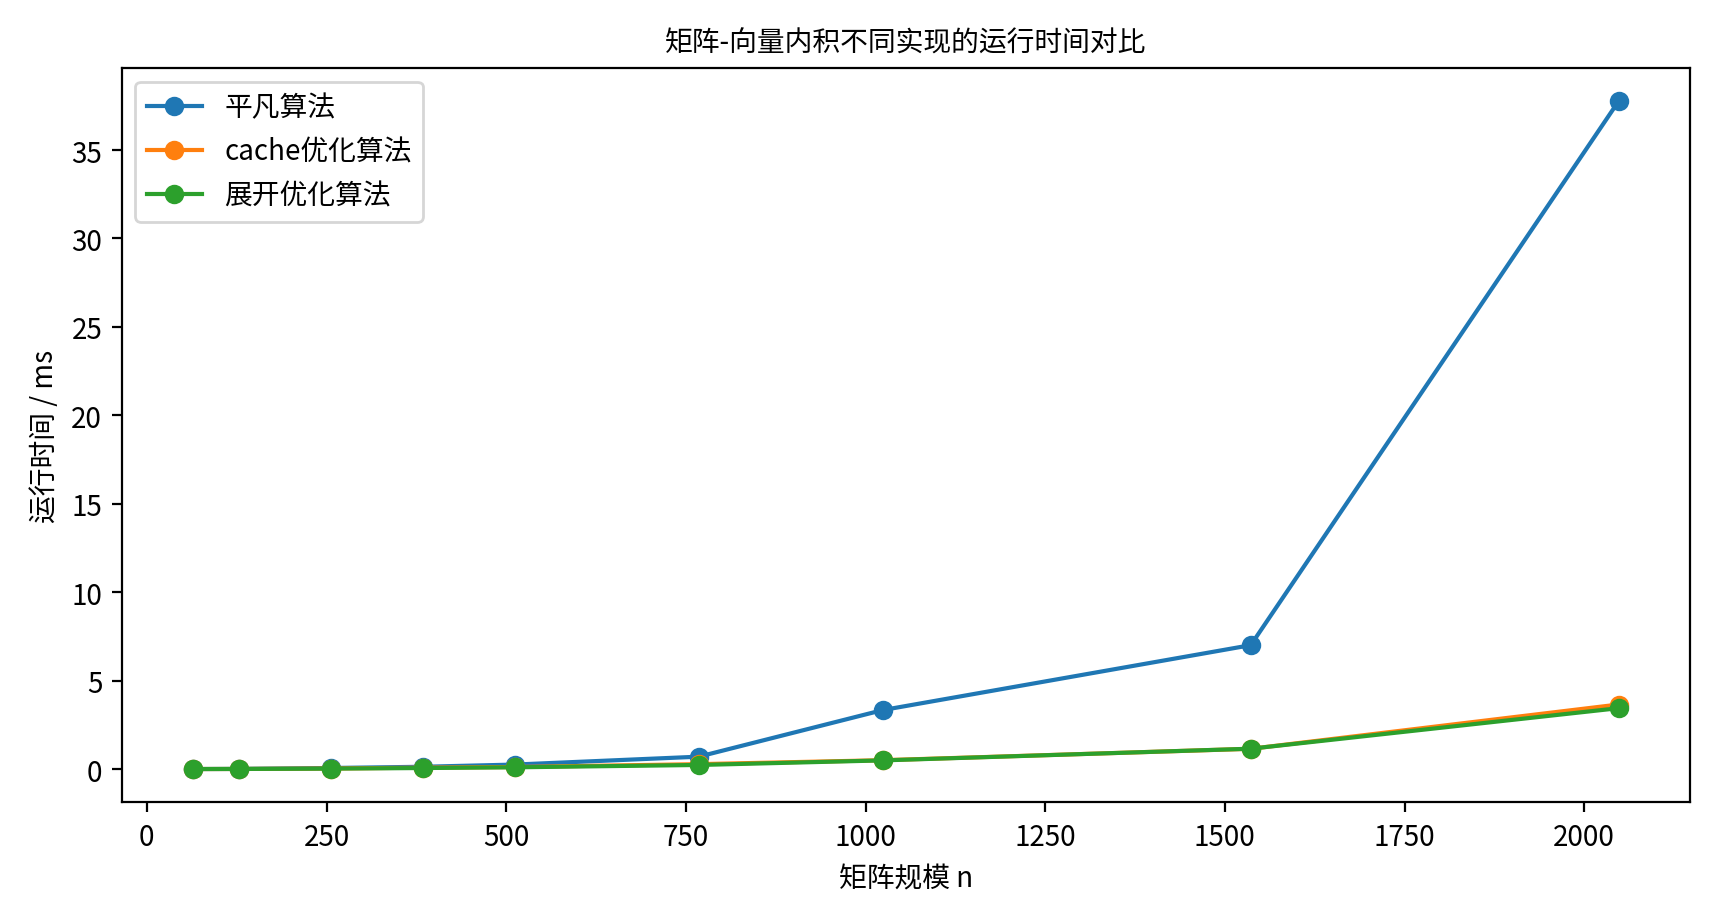
\includegraphics[width=0.92\textwidth]{fig/dot_advanced_integrated.png}
\caption{矩阵内积实验中不同实现版本的运行时间对比}
\label{fig:dot-adv}
\end{figure}

\subsubsection{Godbolt 汇编分析}
为了进一步解释矩阵内积实验中的性能差异，本文利用 Godbolt 对 cache 优化版本函数 \texttt{dot\_cache} 和四路展开版本函数 \texttt{dot\_cache\_unroll4} 在 \texttt{-O2} 条件下生成的汇编代码进行了对比观察。从结果可以看到，前者在进入主计算前先调用 \texttt{memset} 将结果数组清零，随后外层按行推进、内层循环按顺序读取一行矩阵元素并完成标量乘加与写回，其核心指令模式主要表现为 \texttt{movsd}、\texttt{mulsd}、\texttt{addsd} 与循环分支配合执行；这与正文中的按行访问设计相对应。相比之下，四路展开版本把同一计算模式连续展开为四组，地址步长由 8 字节扩大到 32 字节，并在主循环中保留了更多彼此独立的乘加操作，使平均到每个元素上的归纳变量更新和分支判断次数进一步减少。不过与求和实验不同，这一节的主瓶颈仍然首先来自矩阵访问模式本身；因此展开版本虽然也改善了目标代码结构，但它带来的收益仍然建立在顺序流式访存已经成立的前提之上，只能形成次一级提升。这与前文基础测试和补充测试中的结果是一致的。

\begin{figure}[H]
\centering
\begin{minipage}{0.48\textwidth}
    \centering
    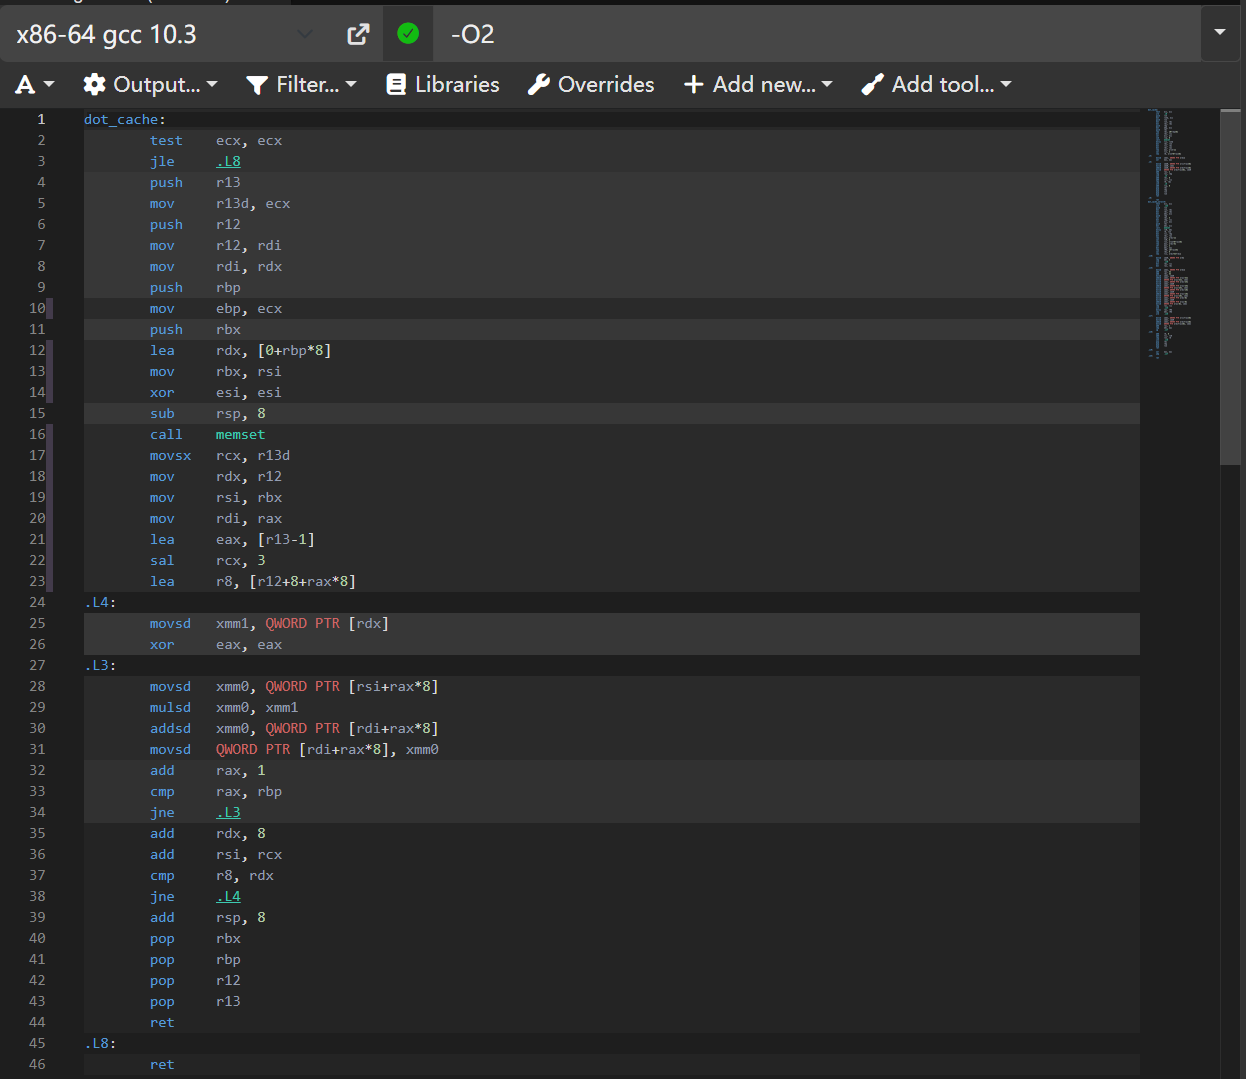
\includegraphics[width=\textwidth]{fig/godbolt_dot_cache_O2.png}
    \\[-0.25em]
    {\scriptsize （a）cache优化版本 \texttt{dot\_cache}}
\end{minipage}
\hfill
\begin{minipage}{0.48\textwidth}
    \centering
    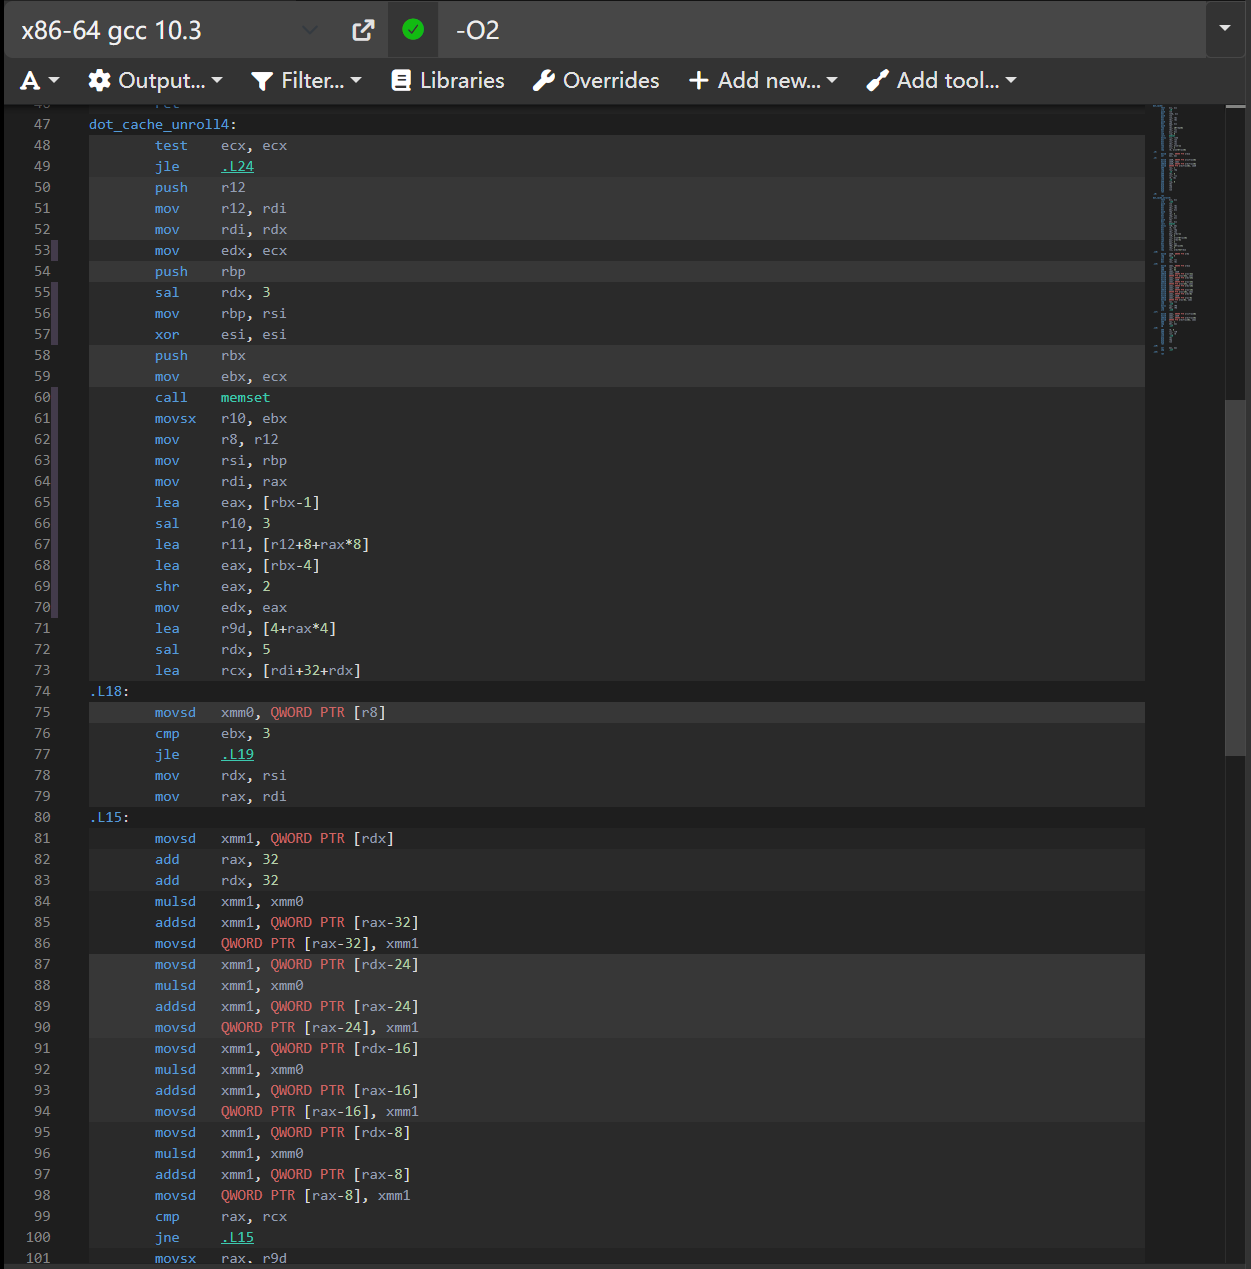
\includegraphics[width=\textwidth]{fig/godbolt_dot_cache_unroll4_O2.png}
    \\[-0.25em]
    {\scriptsize （b）四路展开版本 \texttt{dot\_cache\_unroll4}}
\end{minipage}
\caption{矩阵内积实验中两种优化实现的 Godbolt 汇编对比}
\end{figure}

\section{实验二：$n$ 个数求和}
\subsection{程序设计思路}
第二项任务研究长度为 $n$ 的一维数组求和问题。平凡算法使用单个累加器，从头到尾逐个执行 \texttt{sum += a[i]}。这种写法实现简单，但每一步运算都依赖上一步的结果，会形成一条较长的数据相关链，从而限制处理器流水线和超标量发射单元的并行能力。

优化算法采用两路链式累加的思路：使用两个独立累加器分别处理不同位置的数组元素，最后再把两个部分和相加。这样能够将一条很长的依赖链拆分为两条较短且彼此独立的依赖链，从而更好地发挥处理器的指令级并行能力。在此基础上，又实现了四路展开版本 \texttt{dual\_unroll4}，进一步减少循环控制开销；同时实现了两两归约版本 \texttt{pairwise}，用于观察树形归约结构在串行 CPU 上的实际表现。除运行时间测试外，本文还选取链式累加版本与四路展开版本，通过 Godbolt 观察 \texttt{-O2} 下的汇编结构，以说明依赖链缩短和多累加器设计在目标代码层面的具体体现。

\subsection{实验结果与分析}
\subsubsection{基础测试结果分析}
在 \texttt{-O2} 条件下，链式平凡算法与两路链式累加算法的基础测试结果列于表~\ref{tab:sum-basic}，对应的运行时间变化趋势可结合图~\ref{fig:sum-basic} 观察。由于数据规模从 $2^{10}$ 一直扩展到 $2^{24}$，图中的横轴采用了 $\log_2 n$ 刻度，以便同时观察小规模与大规模区间的差异。基础测试表明，两路链式累加在大多数规模下都优于平凡算法。较典型的是 $n=16384$ 时加速比达到 2.21 倍，在 $n=262144$ 和 $n=1048576$ 时分别为 1.88 倍和 1.89 倍，说明将单累加器改为双累加器后，确实能够缩短数据依赖链并提高指令级并行性。不过当规模增大到 $n=16777216$ 时，加速比下降到 1.04 倍，说明在超大规模下，性能瓶颈已不再主要来自算术依赖，而更多受到内存带宽和整体数据搬移开销的影响。

\begin{table}[H]
\centering
\caption{$n$ 个数求和基础测试结果}
\label{tab:sum-basic}
\scriptsize
\setlength{\tabcolsep}{3pt}
\begin{tabular*}{\textwidth}{@{\extracolsep{\fill}}lccccc@{}}
\toprule
$n$ & 平凡算法时间/ms & 两路链式累加时间/ms & 加速比 & 平凡算法重复次数 & 两路链式累加重复次数 \\
\midrule
1024     & 0.000875 & 0.000533 & 1.639727 & 390624 & 390624 \\
4096     & 0.004069 & 0.002179 & 1.867015 & 97656  & 195312 \\
16384    & 0.016338 & 0.007393 & 2.209832 & 24414  & 48828 \\
65536    & 0.059309 & 0.032988 & 1.797910 & 6102   & 6102 \\
262144   & 0.235940 & 0.125555 & 1.879175 & 1524   & 3048 \\
1048576  & 1.124038 & 0.594254 & 1.891511 & 190    & 380 \\
4194304  & 4.968629 & 3.002182 & 1.655006 & 94     & 94 \\
16777216 & 19.795482 & 19.021014 & 1.040716 & 11    & 22 \\
\bottomrule
\end{tabular*}
\end{table}

\begin{figure}[H]
\centering

\includegraphics[width=0.92\textwidth]{fig/sum_basic_O2.png}
\caption{不同数据规模下链式累加与两路链式累加的运行时间对比（横轴采用 $\log_2 n$ 刻度）}
\label{fig:sum-basic}
\end{figure}

\subsubsection{补充优化结果分析}
进一步地，补充算法与不同编译优化等级下的代表性结果分别列于表~\ref{tab:sum-unroll} 和表~\ref{tab:sum-flags}，图~\ref{fig:sum-adv} 则从整体上呈现了不同实现版本之间的差异。与基础测试图相同，这里横轴同样采用 $\log_2 n$ 刻度，以避免小规模区间的信息被线性坐标压缩。补充结果表明，四路展开版本 \texttt{dual\_unroll4} 的表现明显优于基础的双链路版本 \texttt{dual}。以 $n=1048576$ 为例，双链路版本 \texttt{dual} 用时 0.5943 ms，而展开版本下降到 0.3103 ms，相对平凡算法的加速比提升到 3.62 倍，说明“减少依赖链”和“减少循环控制开销”能够形成叠加收益。相比之下，两两归约版本 \texttt{pairwise} 在串行实现中的表现并不理想：同样在 $n=1048576$ 时，用时达到 2.3392 ms；在 $n=16777216$ 时进一步上升到 59.8760 ms，明显慢于链式与展开版本。这并不意味着它的访存完全无规律，而是因为串行实现需要对同一数组进行多轮扫描：每一轮都要把中间结果写回数组前半段，下一轮再重新读出，导致总内存流量、store 压力和循环层级都明显增加；相较于长期将部分和保存在寄存器中的双链路与展开版本，这类多轮写回会抵消其理论优势。

编译器优化等级对求和实验的影响同样显著。以 $n=1048576$ 为例，平凡版本在 \texttt{-O0}、\texttt{-O2}、\texttt{-O3} 下分别为 3.5348 ms、1.1240 ms 和 0.4229 ms；双链路版本分别为 2.0413 ms、0.5943 ms 和 0.2110 ms。说明在求和这类算术密集型且结构较规则的程序中，编译器优化能够充分发挥作用。当问题规模进一步增大到 $n=16777216$ 时，\texttt{-O3} 仍优于 \texttt{-O2} 和 \texttt{-O0}，但算法之间的差距相对缩小，再次说明大规模情形下访存开销会逐渐削弱单纯依赖算术结构优化所带来的收益。

\begin{table}[H]
\centering
\caption{$n$ 个数求和补充算法的代表性结果（\texttt{-O2}）}
\label{tab:sum-unroll}
\scriptsize
\setlength{\tabcolsep}{2.5pt}
\begin{tabular*}{\textwidth}{@{\extracolsep{\fill}}lccccc@{}}
\toprule
$n$ & 两路链式累加时间/ms & 四路展开时间/ms & 两两归约时间/ms & 两路链式累加加速比 & 四路展开加速比 \\
\midrule
16384    & 0.007393 & 0.004413 & 0.011743 & 2.21 & 3.70 \\
1048576  & 0.594254 & 0.310325 & 2.339208 & 1.89 & 3.62 \\
16777216 & 19.021014 & 16.754614 & 59.875982 & 1.04 & 1.18 \\
\bottomrule
\end{tabular*}
\end{table}

\begin{table}[H]
\centering
\caption{$n$ 个数求和中不同编译优化等级的代表性结果（$n=1048576$）}
\label{tab:sum-flags}
\footnotesize
\setlength{\tabcolsep}{8pt}
\begin{tabular*}{\textwidth}{@{\extracolsep{\fill}}lccc@{}}
\toprule
实现版本 & \texttt{-O0} & \texttt{-O2} & \texttt{-O3} \\
\midrule
平凡版本 & 3.5348 & 1.1240 & 0.4229 \\
双链路版本 & 2.0413 & 0.5943 & 0.2110 \\
\bottomrule
\end{tabular*}
\end{table}

\begin{figure}[H]
\centering
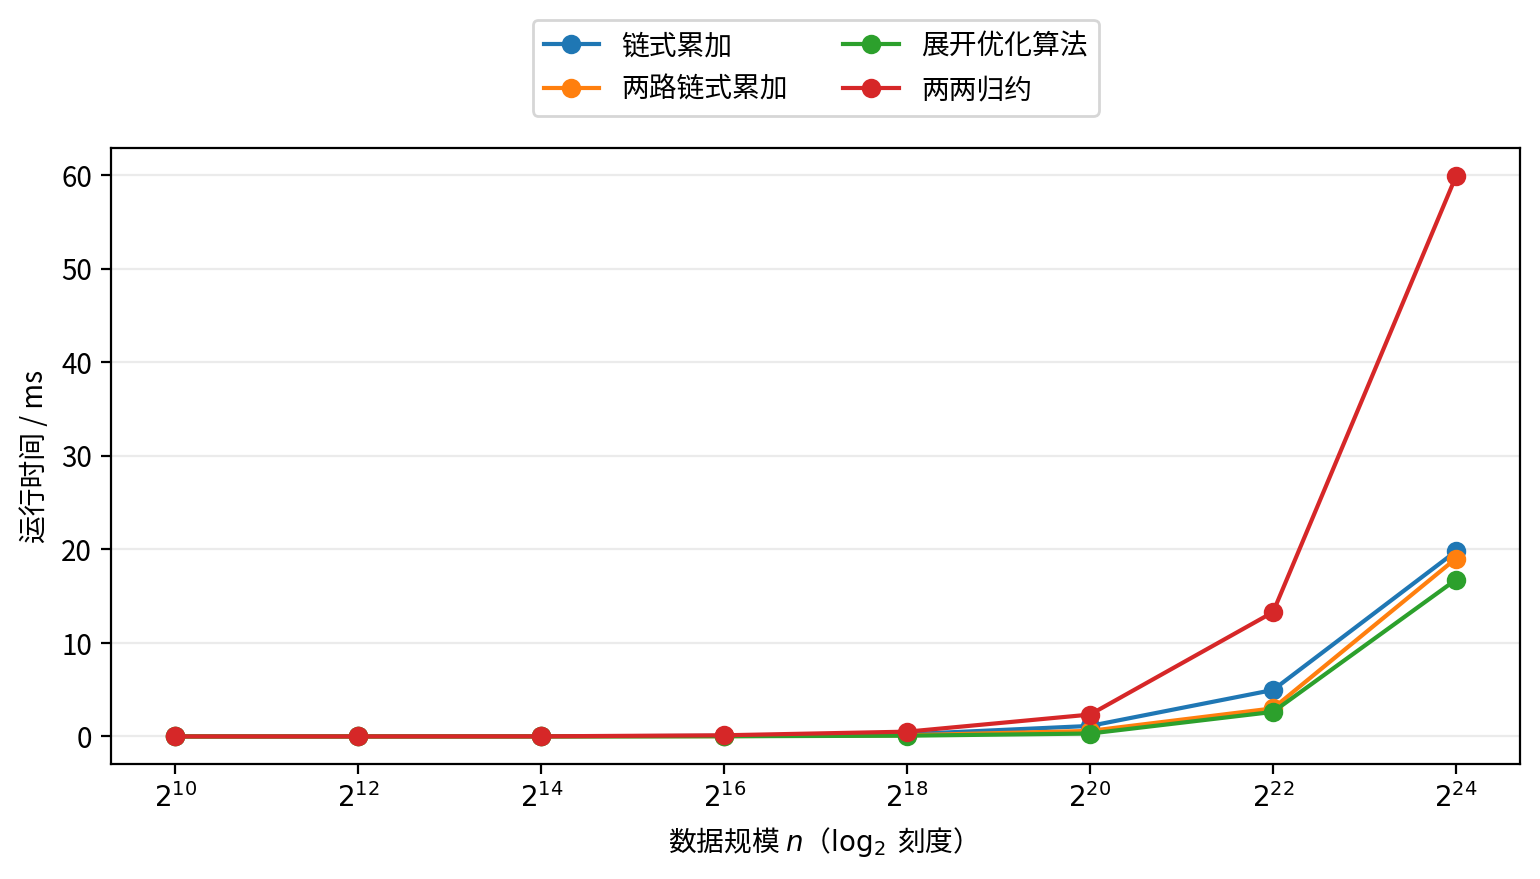
\includegraphics[width=0.92\textwidth]{fig/sum_advanced_integrated.png}
\caption{求和实验中不同实现版本的运行时间对比（横轴采用 $\log_2 n$ 刻度）}
\label{fig:sum-adv}
\end{figure}

\subsubsection{Godbolt 汇编分析}
为了从目标代码层面进一步说明求和实验中的性能差异，本文利用 Godbolt 对链式累加版本函数 \texttt{sum\_naive} 和四路展开版本函数 \texttt{sum\_dual\_unroll4} 在 \texttt{-O2} 条件下生成的汇编代码进行了对比观察。从结果可以看到，链式累加版本的核心循环虽然紧凑，但所有 \texttt{addsd} 都围绕同一个累加寄存器 \texttt{xmm0} 展开，形成了一条连续的 RAW（写后读）依赖链；后一条加法必须等待前一条结果就绪，因此处理器即使具备乱序执行和超标量发射能力，也难以同时推进多条浮点加法。相比之下，四路展开版本在主循环中使用多组寄存器分别保存部分和，一次处理 4 个相邻元素，循环结束后再将多个部分和合并。这意味着循环内部不再只有一条长依赖链，而是被拆成多条彼此独立的短依赖链；当某一条链等待结果写回时，乱序执行引擎仍可将其他已就绪的 \texttt{addsd} 发射到可用执行资源上，从而提升 IPC。分支判断频率的下降确实也有帮助，但相较于打破单累加器 RAW 相关、增加可并行发射的浮点操作，这只是次一级收益。前文中四路展开版本优于链式累加版本的测试结果，正可以由这一汇编层面的差异得到解释；而当数据规模继续增大时，内存访问开销又会逐步抵消这种算术结构优化带来的优势。

\begin{figure}[H]
\centering
\begin{minipage}{0.48\textwidth}
    \centering
    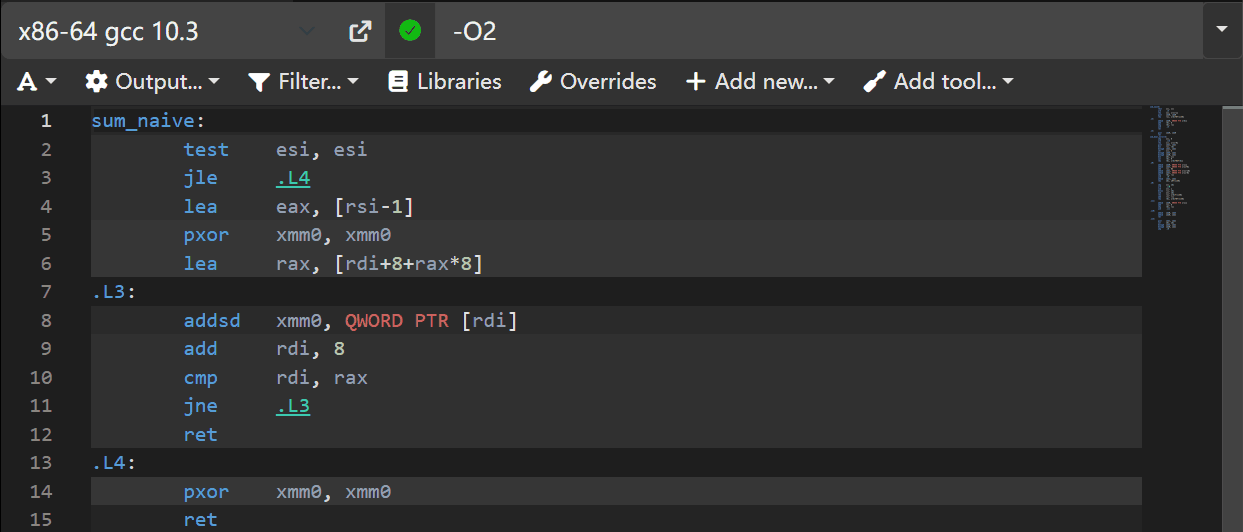
\includegraphics[width=\textwidth]{fig/godbolt_sum_naive_O2.png}
    \\[-0.25em]
    {\scriptsize （a）链式累加版本 \texttt{sum\_naive}}
\end{minipage}
\hfill
\begin{minipage}{0.48\textwidth}
    \centering
    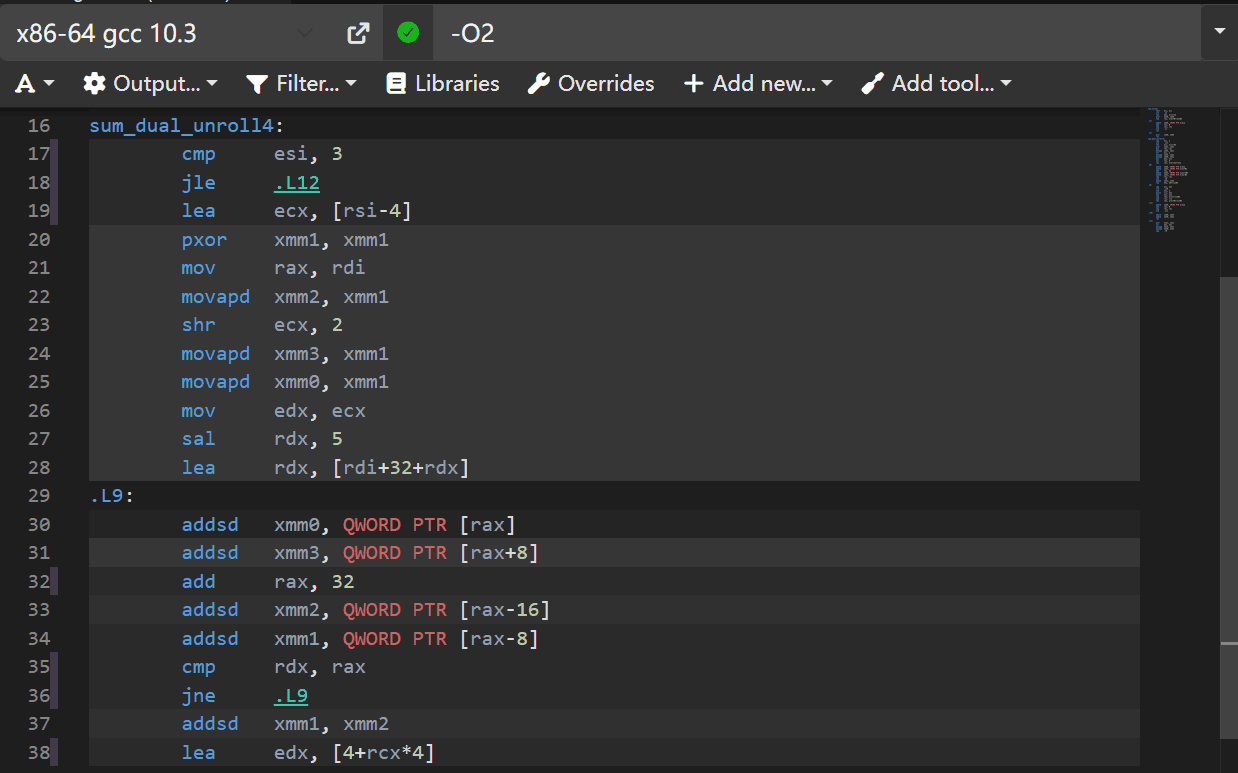
\includegraphics[width=\textwidth]{fig/godbolt_sum_dual_unroll4_O2.png}
    \\[-0.25em]
    {\scriptsize （b）四路展开版本 \texttt{sum\_dual\_unroll4}}
\end{minipage}
\caption{$n$ 个数求和实验中两种实现的 Godbolt 汇编对比}
\end{figure}

\section{实验总结}
本次实验围绕“访存局部性”和“指令级并行”两条主线，完成了矩阵每列与向量内积、$n$ 个数求和两个任务的程序设计、性能测试与结果分析。在矩阵内积部分，本文分别实现了按列访问的平凡算法、按行访问的 cache 优化算法以及四路展开版本，并结合不同问题规模下的重复测试结果进行比较。修正缓存层次的理解后，可以更合理地解释性能拐点：对单线程程序而言，真正重要的是单个核心可利用的缓存，而不是任务管理器显示的全芯片聚合 L1 容量。以 P 核 48 KB L1D 和 2 MB 私有 L2 为参照，平凡算法在行主存储下的跨行步长访存会造成明显的 cache line 浪费；相比之下，cache 优化版本把活跃工作集压缩到“当前行 + 结果向量”，因此当矩阵规模在 $n=512$ 左右接近单核 L2 量级、到 $n=1024$ 以后进一步超出该层缓存时，顺序访问的优势会被明显放大。四路展开和编译器优化则是在这一主访存优化基础上的进一步收益。

在求和部分，本文实现了链式平凡算法、两路链式累加、四路展开版本以及两两归约版本，并比较了不同优化等级下代表性实现的运行时间。结果表明，双累加器与四路展开能够把一条长 RAW 依赖链拆分为多条彼此独立的短链，使乱序执行引擎能够发射更多已就绪的浮点加法，从而提高 IPC，其中四路展开版本在中等规模下表现最优；而两两归约虽然在并行场景中具有一定理论优势，但在当前串行 CPU 上需要进行多轮扫描和中间结果写回，导致总内存流量与 store 压力明显增加，实际效果反而较差。此外，本文还利用 Godbolt 对代表性函数在 \texttt{-O2} 下的汇编结果进行了对比，进一步从目标代码层面验证了前述实验结论：矩阵内积优化的核心在于提高 cache line 利用率并保持较小的活跃工作集，求和优化的核心在于削弱单累加器的 RAW 相关并增加独立累加路径。综合来看，本次实验较为完整地覆盖了基础算法实现、循环展开、编译器优化力度对比、对数坐标下的数据可视化以及 Godbolt 汇编分析等工作，也说明现代处理器上的程序性能不仅取决于算法本身，还深受缓存层次、数据布局、访存顺序、指令依赖关系和编译器生成代码质量的共同影响。

\end{document}
